\chapter{高度优化的HEVC解码器}

新的视频编码标准HEVC虽然显著提高了编码效率,但其复杂度也有了明显的提升。现有的用户设备计算资源有限,如何快速实时的解码成为了HEVC广泛应用于流媒体系统的一个阻碍。在硬件解码芯片普及之前,软件解码器的实现和优化是一项重要且有挑战性的工作。在本章中,我们给出了一个高度优化的HEVC软件解码器,并对其在不同处理器平台上的速度进行了测试。

\section{新的解码器原型设计}

HEVC标准化组织提供的参考软件HM中虽然包含了一个HEVC解码器的实现,但是这个实现主要目的是为了方便标准制定和相关的研究性实验,其结构冗余复杂,解码效率低下,不适合实际使用。为了确保本文后续优化工作的有效性和实用性,我们自行设计了一个新的解码器原型。

\begin{figure}[t]
	\centering
	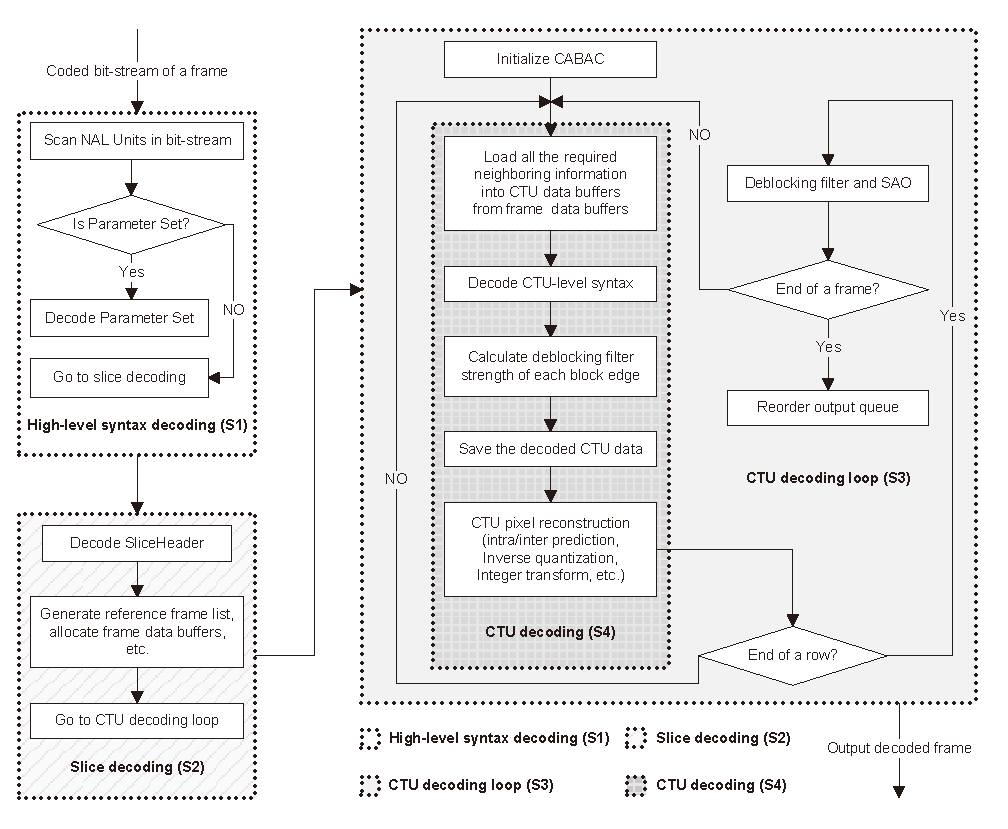
\includegraphics[width = 1.0\linewidth]{eps/decoding_workflow}
	\caption{\label{fig:decoding_workflow}新的解码器原型流程框架}
\end{figure}

该解码器原型的四阶段流程框架如图\ref{fig:decoding_workflow}所示,其中列出了解码器结构中的四个关键阶段,即:高层语法解码、slice解码、CTU\footnote{Coding Tree Unit,HEVC中的基本解码单元,类似H.264/AVC中的宏块}解码循环和CTU解码,对应图中的S1-S4。这个解码器原型有两个不同于HM中参考解码器的特性。第一,在CTU解码(S4)的开始阶段,数据会从全局性的帧缓冲区拷贝一份到CTU缓冲区。这样可以保持这个CTU解码过程中数据访问的局部性,从而降低处理器的缓存失效率。该特性有助于接下来要讨论的单指令多数据(SIMD)优化算法。第二,在CTU解码循环(S3)中,去块滤波和SAO这些理论上要等整帧解完之后才进行的操作,会在每个CTU的像素重建之后立即开始。这样使得这个CTU能够尽早被参考,也就意味着更多的解码任务可以并行执行。该特性为本文后面要介绍的帧级多线程解码框架打下了基础。

需要指出的是,虽然第一个特性有助于提高缓存命中率,但增加了数据拷贝的额外开销。为了尽量减小这一开销,我们会严格选择所需数据:对于当前的CTU解码,只有它上面和左边的CTU可能被用到;而且这两个CTU中有用的分别只是下边界和右边界的数据。按需进行精细复制可以避免大量多余的内存拷贝操作。另外的内存优化还包括对帧缓冲区的处理。所有帧缓冲区都被设计为全局的,只在解码程序开始时统一分配,解码过程中以内存池的方式进行管理,程序运行结束后统一释放。这一机制尽量避免了频繁地内存分配和释放操作,有利于提高程序的内存使用效率和执行速度。

在这一全新的解码器原型基础上,我们接下来用SIMD优化和多线程并行这两种方法来对整个解码过程进行加速。

\section{耗时模块的加速}

大多数现代通用处理器都有SIMD扩展指令集,例如x86架构上的MMX、3DNow!、SSEx、AVX等\supercite{Intel-manual},以及ARM架构上的NEON\supercite{ARM-manual}。这类指令集中的一条指令可以同时操作位于特殊向量寄存器中的多个数据,能成倍地提高数据吞吐率。在这一节中,我们用SIMD技术来加速HEVC解码中的几个耗时模块。

\begin{table}
	\begin{center}
		\caption{HEVC解码过程中各个模块的时间占比} \label{table:HEVC_timing}
		\renewcommand{\arraystretch}{1.5}
		\begin{tabular}{c|c}
			\hline
			\textbf{解码模块} & \textbf{时间占比} \\
			\hline
			\hline
			运动校正 & $47.88\%$ \\
			\hline
			反变换 & $14.5\%$ \\
			\hline
			熵解码 & $12\%$ \\
			\hline
			去块滤波 & $7.76\%$ \\
			\hline
			采样自适应偏移 & $5.12\%$ \\
			\hline
			内存操作 & $5\%$ \\
			\hline
			反量化 & $2.24\%$ \\
			\hline
			其他 & $5.5\%$ \\
			\hline
		\end{tabular}
	\end{center}
\end{table}

根据对HEVC解码过程时间分布的测量统计\supercite{Duan2014},较高码率的码流在解码中各个模块的时间消耗比例如表\ref{table:HEVC_timing}所示。其中耗时较多且适合用SIMD来优化的几个模块包括:运动校正、反变换、去块滤波和采样自适应偏移(熵解码虽然耗时较多,但不适合用SIMD技术进行优化;而且据我们所知没有很好的加速方法)。这几个模块中,运动校正和反变换已经在Yan等人的工作\supercite{Yan-VCIP2012}中被充分地优化过了,本文直接采用其结果;而对于已有工作尚未很好处理的去块滤波和采样自适应偏移,我们将分别设计新的算法对其进行加速。下面介绍的算法对x86架构和ARM架构都适用,在具体实现上有差异的地方我们会单独指出。

\subsection{低复杂度运动补偿插值算法}

在HEVC中,运动补偿的实质是水平和竖直方向的插值操作,每个方向的插值过程均采用8抽头DCT插值滤波器插值得到目标亮度分量,并采用4抽头DCT插值滤波器插值得到目标色度分量。无论是水平还是竖直方向的插值,DCT插值滤波器的插值过程均可表示为如下形式:
\begin{equation}\label{equ:formula-DCT-IF}
Component_{luma} = \sum_{m=0}^7 p_m \times L_m \quad \texttt{以及} \quad Component_{chroma} = \sum_{m=0}^3 q_m \times C_m,
\end{equation}
其中$L_0 - L_7$和$C_0 - C_3$分别代表亮度与色度的原始输入像素,$p_0 - p_7$和$q_0 - q_3$分别代表相应的滤波器系数组 (groups of interpolation coefficients) 。对于亮度分量,运动补偿插值的精度为$1/4$像素,对于色度分量,运动补偿插值的精度为$1/8$像素,因此不论是水平还是竖直方向插值,与其精度相对,亮度分量有$4$个不同的位置,色度分量则有$8$个不同的位置。以水平插值为例,亮度分量与色度分量各自的位置分别如图\ref{fig:luma_position}和图\ref{fig:chroma_position}所示,其对应的插值系数组如表\ref{table:coeff_position}所示。根据式(\ref{equ:formula-DCT-IF})和表\ref{table:coeff_position},无论水平还是竖直方向插值,得到一个亮度分量需要执行多达$72$次乘法操作,代表了运动补偿中主要的耗时来源。

\begin{table}[!tp]
	\begin{center}
		\caption{HEVC运动补偿的插值系数组} \label{table:coeff_position}
		\renewcommand{\arraystretch}{1.3}
		\begin{tabular}{c|p{1cm}|p{1cm}|p{1cm}|p{1cm}|p{1cm}|p{1cm}|p{1cm}|p{1cm}}
			\hline
			\textbf{亮度分量位置} & \textbf{$p_0$} & \textbf{$p_1$} & \textbf{$p_2$} & \textbf{$p_3$} & \textbf{$p_4$} & \textbf{$p_5$} & \textbf{$p_6$} & \textbf{$p_7$} \\
			\hline
			\hline
			$L_3$ & $0$ & $0$ & $0$ & $64$ & $0$ & $0$ & $0$ & $0$ \\
			\hline
			$a$ & $-1$ & $4$ & $-10$ & $58$ & $17$ & $-5$ & $1$ & $0$ \\
			\hline
			$b$ & $-1$ & $4$ & $-11$ & $40$ & $40$ & $-11$ & $4$ & $-1$ \\
			\hline
			$c$ & $0$ & $1$ & $-5$ & $17$ & $58$ & $-10$ & $4$ & $-1$ \\
			\hline
			\hline
			\textbf{色度分量位置} & \multicolumn{2}{|c|}{\textbf{$q_0$}} & \multicolumn{2}{c}{\textbf{$q_1$}} & \multicolumn{2}{|c|}{\textbf{$q_2$}} & \multicolumn{2}{c}{\textbf{$q_3$}} \\
			\hline
			\hline
			$C_1$ & \multicolumn{2}{|c|}{\textbf{$0$}} & \multicolumn{2}{c}{\textbf{$64$}} & \multicolumn{2}{|c|}{\textbf{$0$}} & \multicolumn{2}{c}{\textbf{$0$}} \\
			\hline
			$d$ & \multicolumn{2}{|c|}{\textbf{$-2$}} & \multicolumn{2}{c}{\textbf{$58$}} & \multicolumn{2}{|c|}{\textbf{$10$}} & \multicolumn{2}{c}{\textbf{$-2$}} \\
			\hline
			$e$ & \multicolumn{2}{|c|}{\textbf{$-4$}} & \multicolumn{2}{c}{\textbf{$54$}} & \multicolumn{2}{|c|}{\textbf{$16$}} & \multicolumn{2}{c}{\textbf{$-2$}} \\
			\hline
			$f$ & \multicolumn{2}{|c|}{\textbf{$-6$}} & \multicolumn{2}{c}{\textbf{$46$}} & \multicolumn{2}{|c|}{\textbf{$28$}} & \multicolumn{2}{c}{\textbf{$-4$}} \\
			\hline
			$g$ & \multicolumn{2}{|c|}{\textbf{$-4$}} & \multicolumn{2}{c}{\textbf{$36$}} & \multicolumn{2}{|c|}{\textbf{$36$}} & \multicolumn{2}{c}{\textbf{$-4$}} \\
			\hline
			$h$ & \multicolumn{2}{|c|}{\textbf{$-4$}} & \multicolumn{2}{c}{\textbf{$28$}} & \multicolumn{2}{|c|}{\textbf{$46$}} & \multicolumn{2}{c}{\textbf{$-6$}} \\
			\hline
			$i$ & \multicolumn{2}{|c|}{\textbf{$-2$}} & \multicolumn{2}{c}{\textbf{$16$}} & \multicolumn{2}{|c|}{\textbf{$54$}} & \multicolumn{2}{c}{\textbf{$-4$}} \\
			\hline
			$j$ & \multicolumn{2}{|c|}{\textbf{$-2$}} & \multicolumn{2}{c}{\textbf{$10$}} & \multicolumn{2}{|c|}{\textbf{$58$}} & \multicolumn{2}{c}{\textbf{$-2$}} \\
			\hline
		\end{tabular}
	\end{center}
\end{table}

\begin{figure}[!tp]
	\centering
	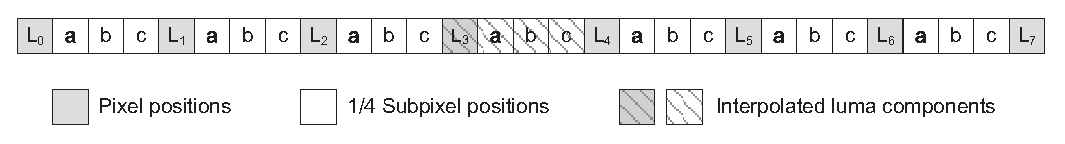
\includegraphics[width = 0.95\linewidth]{eps/luma_position}
	\caption{\label{fig:luma_position}
		HEVC运动补偿亮度分量水平插值采用的8抽头DCT插值滤波器}
	% \vspace{5pt}
\end{figure}

\begin{figure}[!tp]
	\centering
	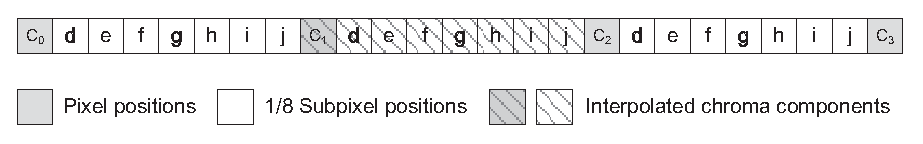
\includegraphics[width = 0.95\linewidth]{eps/chroma_position}
	\caption{\label{fig:chroma_position}
		HEVC运动补偿色度分量水平插值采用的4抽头DCT插值滤波器}
	% \vspace{5pt}
\end{figure}

DCT插值滤波的过程是典型的向量乘法,针对水平和竖直方向插值的不同特点,本文提出了不同的SIMD数据级并行算法来实现降低运动补偿乘法的复杂度的优化目的。水平插值的算法实现是建立在本文之前的工作的基础上,该方案以极高的寄存器利用率可达到同时插值多达8个亮度分量的并发度,算法的核心部分如图\ref{fig:DCT-IF_luma}所示,其流程如下。首先滤波器系数组$p_0 - p_7$分两次载入向量寄存器$R_0$,然后将原始像素$L_0 - L_{14}$载入向量寄存器$R_1$。为了最大化寄存器利用率,$R_1$中的15个像素以交织排列的方式载入向量寄存器$R_2 - R_5$,从而仅使用4条PMADDUBSW指令、3条PHADDW指令以及1条MOVDQA指令即可在寄存器$R_2$中同时得到8个插值完毕的16比特亮度分量,平均到每个亮度分量的插值仅需要$1/2$条PSHUFB指令、$1/2$条PMADDUBSW指令、$3/8$条PHDDW指令以及$1/8$对load/store操作,使得指令数目以及访存次数均得到了有效控制。

对于竖直方向的插值算法,PMADDUBSW指令不再适用,在本文之前的工作中,采用了迭代进行乘法与加法的直观算法,在这种情况下得到一个插值完毕的亮度分量平均需要$1$条乘法指令与$7/8$条加法指令。而本文则提出了全新的无乘法SIMD运动补偿的竖直方向插值算法设计方案,能够进一步减少指令执行周期并且实现多达16个亮度分量的同时插值。新算法的基本设计思想是从向量乘法中抽取可最大限度重用的公共运算单元,并借助公共运算单元将向量乘法拆分成最小的加法、减法和移位运算集合。举例来说,针对亮度分量位置$a$与$b$的DCT插值滤波操作可被重构为:
\begin{eqnarray}
component_{luma,a} &=& T_0 + ((T_0+L_1)<<2) + (L_3<<5)
\nonumber 
\\&& + L_4 + ((L_3+L_4)<<4)- L_0 + L_6,
\end{eqnarray}
以及
\begin{eqnarray}
component_{luma,b} &=& ((L_1+L_6)<<2) - (L_0+L_7)
\nonumber 
\\&& - T_1 + T_2 + (T_2<<2),
\end{eqnarray}
其中,$T_0 = ((L_3 - L_2)<<1)$,$T_1 = L_2 + L_5$,$T_2 = ((L_2 + L_5)<<3) - (T_1<<1)$ 均为公共运算单元。类似地,针对色度分量位置$d$、$e$、$f$与$g$的DCT插值滤波操作可被重构为:
\begin{eqnarray}
component_{chroma,d} &=& (C_1<<4) + (C_1<<5) + (T_3<<3)
\nonumber 
\\&& + ((T_3 - C_0 - C_3)<<1),
\end{eqnarray}
\begin{eqnarray}
component_{chroma,e} &=& (C_1<<5) + ((C_1+C_2)<<4) 
\nonumber 
\\&& + ((C_1-C_0)<<2) + ((C_1-C_3)<<1),
\end{eqnarray}
\begin{eqnarray}
component_{chroma,f} &=& (C_1<<3) + ((C_1+C_2)<<5) 
\nonumber 
\\&& + (T_1<<4) + ((T_4-C_2-C_3)<<2),
\end{eqnarray}
以及
\begin{equation}
component_{chroma,g} = (T_3<<5) + ((T_3-C_0-C_3)<<2), 
\end{equation}
其中$T_3 = C_1 + C_2$以及$T_4 = C_1 - C_0$均为公共运算单元。对于亮度分量位置$c$以及色度分量位置$h$、$i$、$j$,其重构成公共运算单元最小运算集合的方法分别与亮度分量位置$a$以及色度位置分量位置$f$、$e$、$d$完全对称。此处不再赘述。对于亮度分量位置$L_1$和色度分量位置$C_1$,采用最简单的移位运算代替乘法运算即可。采用上述的新算法之后,为了获得一个位置为$a$或$c$插值完毕的亮度分量平均仅需要$1/2$条移位指令、$3/8$条减法指令以及$7/8$条加法指令,而对于位置为$b$的插值完毕的每个亮度分量平均仅需要$1/2$条移位指令、$3/8$条减法指令以及$3/4$条加法指令。与之前工作中直观的SIMD算法相比,无论是指令数目还是指令的复杂度均有所下降,因此整体的指令执行周期得到了进一步的优化。类似的结论也可通过对色度分量的插值运算的分析而得到。

\begin{figure}[!tp]
	\centering
	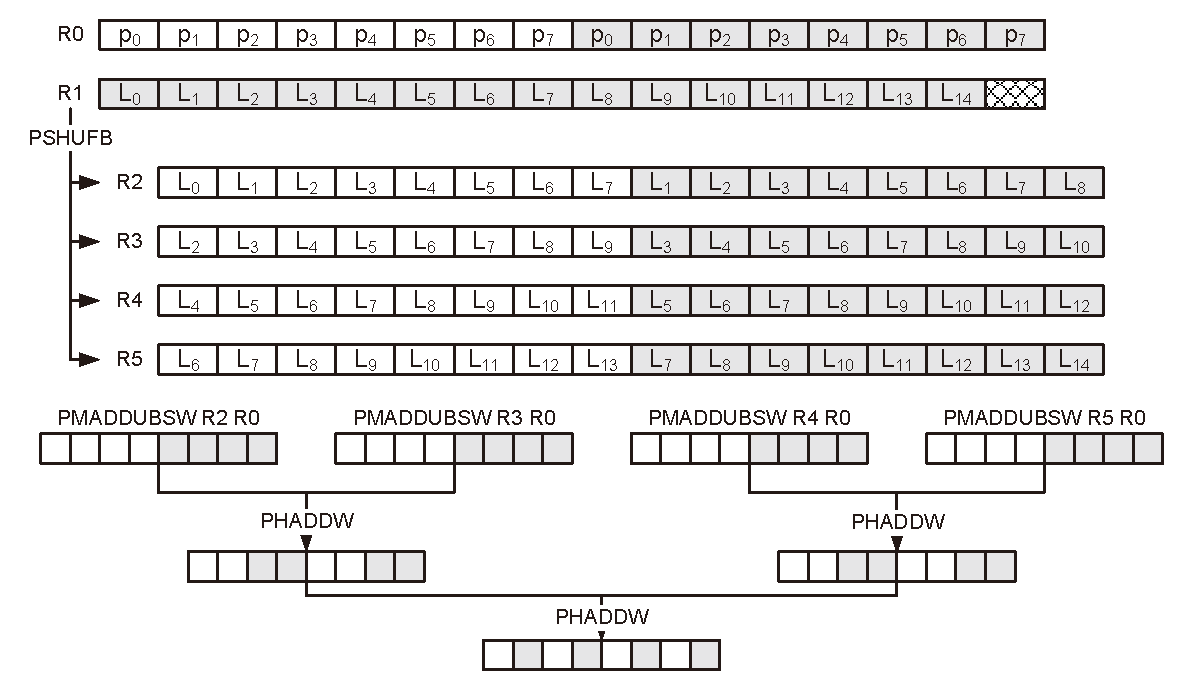
\includegraphics[width = 0.95\linewidth]{eps/DCT-IF_luma}
	\caption{\label{fig:DCT-IF_luma}
		低复杂度运动补偿的水平插值算法,实现8个亮度分量的并行插值}
	% \vspace{5pt}
\end{figure}

综上所述,通过本节提出的全新SIMD数据级并行算法,运动补偿模块的水平插值与竖直方向插值运算的并行度得到了大幅提升,并且指令执行周期和访存次数进一步缩减,预期将取得显著的加速比,从而为整个解码流程节省可观的执行时间。

\subsection{无转置反变换算法}\label{sec:6.3.4}
在H.265/HEVC中,整数变换的实质依旧是矩阵乘法,在解码阶段,反变换可表示为如下形式:
\begin{equation}
R = T^TXT,
\end{equation}
其中$T$是变换系数矩阵,$X$是经过反量化之后的残差系数矩阵,$R$为反变换结果矩阵。在本文之前的工作中,反变换的SIMD并行算法设计采用先列变换再行变换的两阶段实现方式:
\begin{equation}\label{equ:formula-transform-step1}
Step1:	\quad B_{i,j} = \sum_{k=0}^n A_{i,k}X_{k,j},
\end{equation}
以及
\begin{equation}\label{equ:formula-transform-step2}
Step2:	\quad R_{i,j} = \sum_{k=0}^n B_{i,k}A_{j,k},
\end{equation}
其中$B$为保存中间结果的矩阵,$A$代表$T^T$为变换系数矩阵的转置。由式(\ref{equ:formula-transform-step1})与式(\ref{equ:formula-transform-step2})可知,即便矩阵$A$可以通过提前预取放置在寄存器中,矩阵$X$依然需要通过转置才能够有效地按行方式将列数据读入向量寄存器,然后才可进行列变换操作。转置的过程不仅仅会产生大量的指令数目以及访存的时间开销,而且还会大量占用向量寄存器资源,降低可用于计算的向量寄存器数量,从而对数据级并行度造成不良影响,因此将转置操作从变换过程中移除是十分必要的。

为了达到从反变换中移除转置的目标,本文采用了一种全新的设计思路,通过对整数变换过程的重新梳理实现矩阵乘法与转置操作的解耦合,从而将转置操作打散并恰当地融入列变换的过程中。图\ref{fig:transpose-free_IT}中展示了算法的核心过程,以计算$32 \times 32$大小的变换单元TU的中间结果矩阵$B$的前四个系数的过程为例,其关键在于预取之后的数据排布顺序:当系数矩阵$A$的每一行系数两两进行了置乱 (shuffle) 操作并且中间结果矩阵$B$的每两行系数按照相应顺序完成交织排布之后,即可进行高效的向量乘法运算。对于大小为$N \times N$ ($N = 8, 16, 32$) 的变换单元TU,中间结果矩阵$B$每次可以并行得到4个列变换之后的系数,消耗$N/2$条PMADDWD指令以及$N/2 - 1$条PADDD指令,得到的中间结果系数为32比特长度,经过打包 (pack) 操作之后即可直接用于行变换的计算,无需任何多余的转存或转置操作,从而有效地减少了指令数目并且使寄存器得到了更有效的利用。由于所有存放矩阵系数的缓冲区均已按照16-byte进行了首地址对齐,从内存中预取系数矩阵的访存开销也已降至最低。

\begin{figure}[!tp]
	\centering
	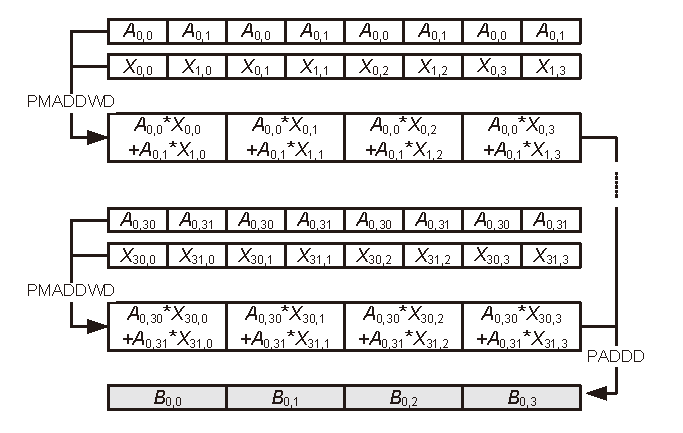
\includegraphics[width = 0.8\linewidth]{eps/transpose-free_IT}
	\caption{\label{fig:transpose-free_IT}
		无转置反变换算法的核心过程,以计算中间结果矩阵$B=AX$的前四个系数为例}
	% \vspace{5pt}
\end{figure}

另一方面,可能存在的疑问是\ref{sec:6.3.3}节针对运动补偿插值设计的低复杂度算法能否用于反变换过程中用简单的加减和移位运算取代乘法操作。需要指明的是,在H.265/HEVC中,每个不同大小的变换单元TU其变换系数矩阵都是不同的,因此难以找到能够被多次重复使用的公共运算单元,在此种情况下若采用类似\ref{sec:6.3.3}节的方法对反变换的向量乘法进行拆分将反而导致指令数目的急剧上升以及执行效率的下降。另外同样需要指出的是,有限的向量寄存器个数依然是限制反变换的SIMD数据级并行算法性能的瓶颈,对于$16 \times 16$以及$32 \times 32$大小的变换单元TU不得不通过多次装载数据的方式才可分批完成整个反变换过程,这一瓶颈有望在64位系统上通过采用新的SIMD多媒体指令集如AVX2的方式,借助更多的向量寄存器以及更大的数据吞吐量得到缓解。

\subsection{对称去块滤波算法}

在HEVC的去块滤波中,对于8x8的块边界,每次以4个像素为单元来决定是否需要进行滤波,并决定是进行高强度滤波还是普通滤波。这样就把边界同一侧每次操作的像素个数限制为4,无法充分利用向量寄存器同时对8个像素进行计算。为了提高并行度,我们设计了一个与Yang等人在H.264/AVC解码器优化工作\supercite{Yang-TCE2006}中的描述类似的对称去块滤波算法。

\begin{figure}[h]
	\centering
	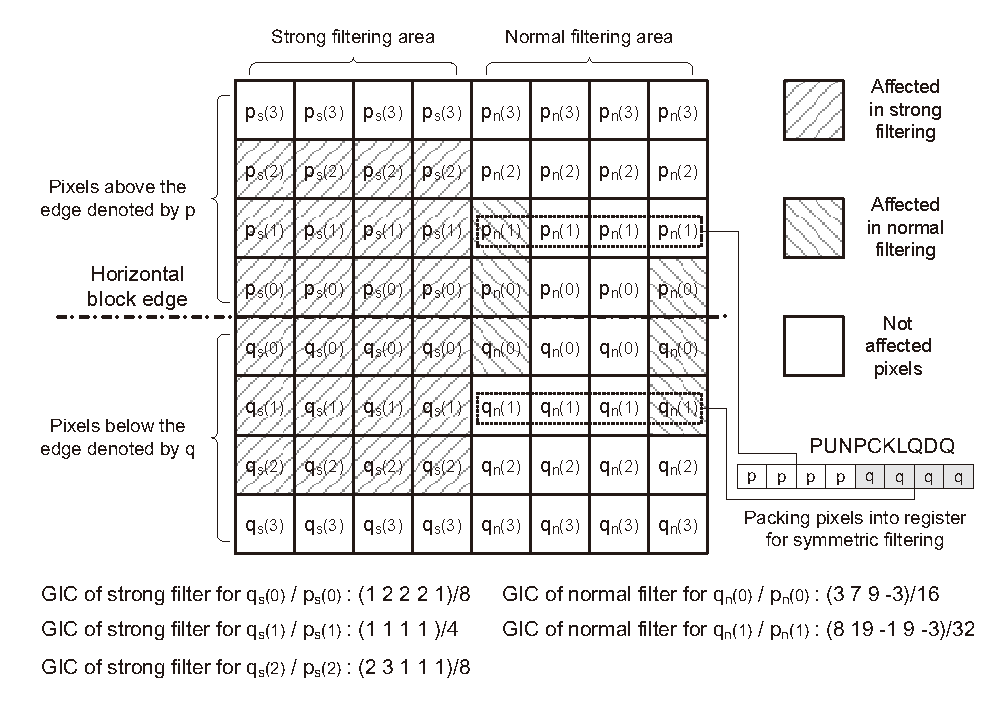
\includegraphics[width = 1.0\linewidth]{eps/vertical_DF_to_horizontal_edge}
	\caption{\label{fig:vertical_DF_to_horizontal_edge}HEVC中对$8 \times 8$块的水平边界进行滤波的操作示意图}
\end{figure}

图\ref{fig:vertical_DF_to_horizontal_edge}展示的是HEVC标准中对8x8块的水平边界进行滤波的操作示意图。滤波操作实质上就是对边界两侧的像素进行修改。在每侧的4个像素中,高强度滤波会修改其中的3个,普通滤波会修改其中的2个或1个或0个。修改的方法可以认为是一个插值的过程。原来的像素会被改为用它上下的像素进行插值(加权平均)的结果,从而实现像素值的平滑,达到消除边界的目的。在图\ref{fig:vertical_DF_to_horizontal_edge}所示的例子里,左边四列像素进行的是高强度滤波,右边四列是普通滤波。图的下方列出了对各个像素进行修改时用到的插值系数组(group of interpolation coefficients,简称GIC),相当于滤波器的冲激响应\supercite{Norkin-TCSVT2012}。这里有一个比较关键的地方在于,根据HEVC对滤波模块的规定,边界两侧相同位置的像素,其GIC是一样的,而且插值所用的像素也是对称的。利用这个性质,我们可以用PUNPCKLQDQ这一SIMD指令把边界两侧相同位置的像素放在一个寄存器里同时参与计算。如图\ref{fig:vertical_DF_to_horizontal_edge}中所示,在高强度滤波中,对于0~3的每一个$i$,标记为$p_n(i)$的4个像素和标记为$q_n(i)$的4个像素放在一起;同样的,在普通滤波中,对于0~3的每一个$j$,标记为$p_s(j)$的4个像素和标记为$q_s(j)$的4个像素放在一起。这样,无论是哪种滤波方式,每次能处理8个像素,充分利用了128位向量寄存器(在滤波操作中因为要存储中间值,每个像素需占用16位),使得滤波操作所需的指令数减少了一半。

对于普通滤波方式来说,因为受影响的像素数不确定(0个到2个都有可能),所以在与高强度滤波同样的方式计算出滤波结果之后,还要另外用某种阈值来决定哪些像素最终会被滤波结果取代。这时可以用阈值来构造掩模,用掩模去选择最终结果。例如,对于图\ref{fig:vertical_DF_to_horizontal_edge}中的$q_n(0)$和$p_n(0)$行,中间两个像素不受影响,所以其4 x 16bit掩模应为:
\begin{equation}
Mask = \{ \texttt{0xffff}, \quad \texttt{0}, \quad \texttt{0}, \quad \texttt{0xffff} \}.
\end{equation}
基于此,普通滤波的最终结果可确定为:
\begin{equation}
ResultRow = (OriginalRow \land \neg Mask ) \lor (FilteredRow \land Mask).
\end{equation}
这些操作可以用并行逻辑运算指令PAND、PANDN以及POR很轻易地实现。

上面讨论的是水平边界的滤波。对于竖直边界,该算法过程是一致的,只需要先进行一次转置,然后按照上述方法进行计算即可。

\subsection{并行索引SAO算法}

在HEVC解码中,去块滤波之后的像素需要先进行采样自适应偏移(SAO)才能输出为解码图像。对于每个CTU,其像素进行SAO的模式由码流中解析出的\textit{SAOType}来指定。SAO模式有两种,一个是条带(Band)模式,一个是边缘(Edge)模式。这两种模式都会在原像素值上增加一个偏移量。不同之处在于,在条带模式中,这个偏移量由原像素值本身(0~255)来索引,而在边缘模式中,这个偏移量由原像素与其两个相邻像素的梯度值来索引。在条带模式中,每个条带横跨的像素值为4,因此256个不同像素值被分为了32个条带,作为索引去查表决定加到该像素上的偏移量。这样的索引操作在ARM架构上可以用NEON指令集扩展中的并行查表指令进行优化。然而遗憾的是,x86架构下没有对应的指令,只能用普通代码实现。相比于条带模式,边缘模式更为复杂,也是本节提出的并行索引SAO算法主要针对的一种模式。下面进行详细介绍。

\begin{figure}[t]
	\centering
	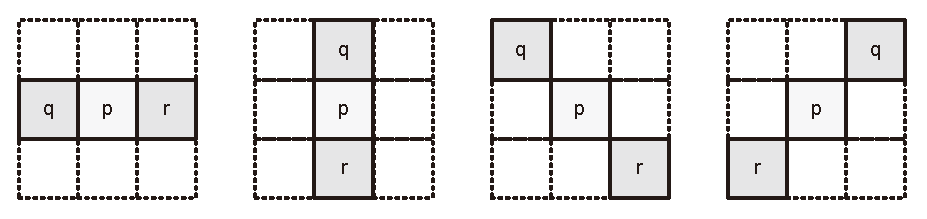
\includegraphics[width = 0.9\linewidth]{eps/SAO_edge_direction}
	\caption{\label{fig:SAO_edge_direction}HEVC中的SAO在边缘模式下选取相邻像素的4种方向}
\end{figure}

\begin{figure}[t]
	\centering
	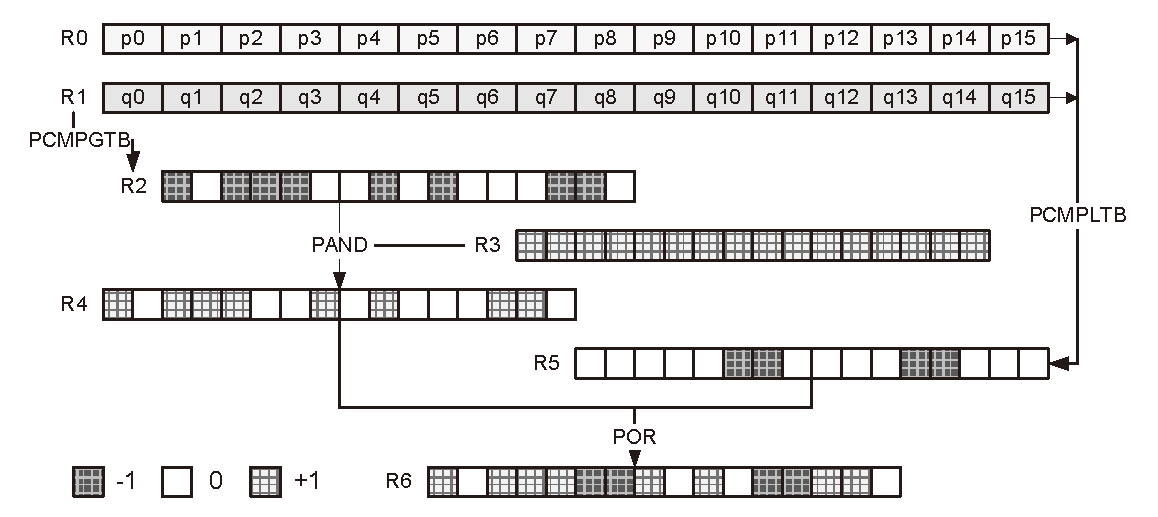
\includegraphics[width = 0.95\linewidth]{eps/SAO_edge_parallel_index}
	\caption{\label{fig:SAO_edge_parallel_index}HEVC中的SAO在边缘模式下的得到16个符号值的过程}
\end{figure}

在边缘模式中,一个像素要减去与它相邻的两个像素。这两个邻居所在的方向可以从图\ref{fig:SAO_edge_direction}中的四个方向选择其一。相减得到两个差值,差值根据其正负或0对应到1、-1和0这三个符号;将两个差值对应的符号相加(可能的结果为-2、-1、0、1、2),作为偏移量的索引。因为一个CTU中的所有像素相减方向都相同,所以计算索引的操作可以并行执行。对于128位的向量寄存器来说,一次可以处理16个像素。图\ref{fig:SAO_edge_parallel_index}展示了我们设计的并行索引算法的核心过程,其中用一对PCMPGTB/PCMPLTB指令和一对PAND/POR指令得到了16个像素相减的符号值。根据选定的方向求出两组符号值之后,通过PADDB指令将它们相加就得到16个索引值,最后用一条PSHUFB指令来查表得到所需的偏移量。很明显这种并行索引SAO算法已经取得了最大的数据级并行度,指令数量已经压缩到最少。需要指出的是,对于图\ref{fig:SAO_edge_direction}中$0^\circ$、$45^\circ$和$135^\circ$这三个方向的相减,将正确的像素取到向量寄存器中会有无法避免的开销,因为要访问的内存是非连续的。


需要指出的是,对于一些比较老的x86机器,其处理器只支持较早期版本的指令集扩展(如SSE2、SSE或MMX),因此上面优化中用到的一些高级指令(如PHADDW、PMADDUBSW等)可能无法使用。为了兼容性考虑,在检测到这样的机器时,一些横向的并行数据操作必须用所支持的较简单指令来实现,这时会有一定的速度牺牲。相反,对于某些支持AVX的最新处理器,向量寄存器的长度由128位扩展到了256位,数据吞吐率可以再提高一倍,这样就能进一步加速这些采用SIMD进行优化的模块。同理,在移动设备上ARM处理器提供的向量寄存器的个数更多,而且SIMD指令集更加智能(能很容易实现转置操作和条带模式SAO中的并行索引),这都能作为速度提升的空间。

总之,在我们所提出的解码器原型基础上,SIMD算法被用于优化大多数耗时解码模块,显著提高了其运行效率。在下一节中,我们将给出一个基于帧的并行解码框架,作为解码器优化的最后一步。

\section{帧级并行解码框架}

\begin{figure}[ht]
	\centering
	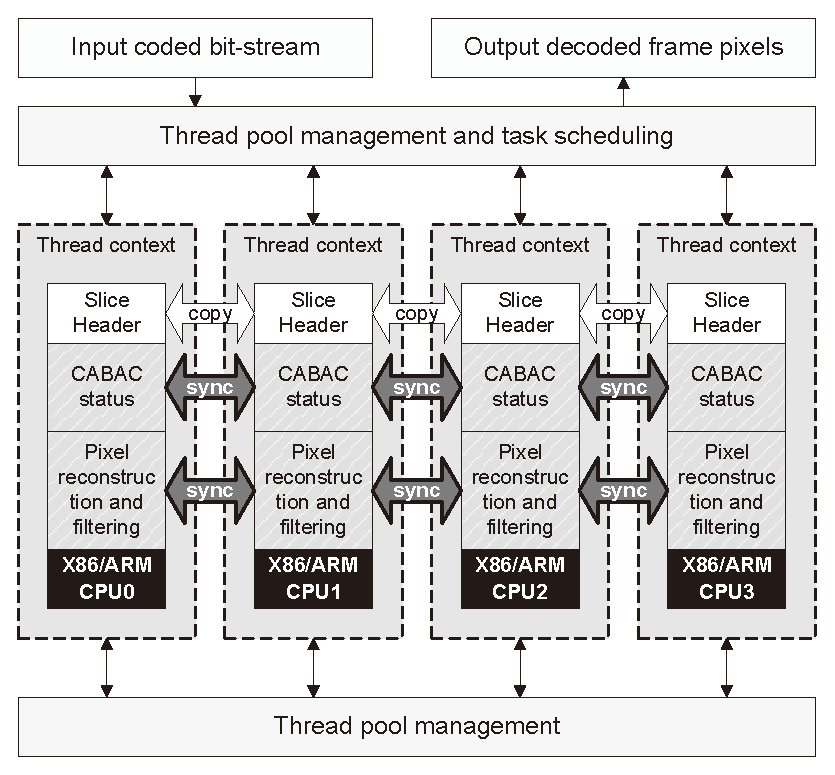
\includegraphics[width = 0.8\linewidth]{eps/parallel_decoding_framework}
	\caption{\label{fig:parallel_decoding_framework}HEVC帧级并行解码框架图}
\end{figure}

随着多核处理器的普及,并行算法成为了发挥这些处理器能力的必需。在本节中,我们提出了一个帧级的并行解码框架,可以在通过多线程取得几倍的解码加速比。该框架如图\ref{fig:parallel_decoding_framework}所示,其工作流程说明如下:
\begin{enumerate}
	\item 首先是解码器初始化;然后在收到码流数据时,入口线程(即主线程)调度第一个可用线程开始解码。
	\item 当第一个可用线程收到码流后,它立即完成slice解码(即图\ref{fig:decoding_workflow}中的S2阶段),并先向主线程发送解码上下文准备好的信号,然后才进入CTU解码循环(即图\ref{fig:decoding_workflow}中的S3阶段)。
	\item 主线程收到解码上下文准备好的信号后,它会把解码上下文信息拷贝到其他可用线程,并调度它们并行地开始后续帧的CTU解码循环。
\end{enumerate}

从该流程和图\ref{fig:parallel_decoding_framework}可以看出,所谓的并行任务指的是不同帧的CTU解码循环及CTU解码过程可以并发地执行,但高层语法和每一帧的slice解码阶段还是需要按照特定的顺序进行。

在本文提出的帧级并行解码框架中,帧内预测的帧是相对独立的,其解码过程与单线程一样。但对于帧间预测的帧,由于运动校正依赖于参考帧的重建像素,所以必须设立线程同步机制。为了平衡同步开销和并发任务的粒度,该框架使用了像素行级别的同步点。对每一帧,有一个变量用于指示该帧的哪一行已经完成解码重建。参考它的帧通过不断检查这一变量,就能在其所依赖的像素行准备好后立即开始进行运动校正。这样的设计用较小的开销解决了解码中的数据依赖问题,提高了潜在的并行度。

\section{优化结果}

在本节中,我们通过详尽的解码速度测试数据来展示整体优化结果。

对于x86架构平台,我们选用了Intel i7-2600 3.4GHz四核处理器,机器内存8GB,操作系统为Microsoft Windows 7。HEVC标准测试序列用HM 10编码器编码,重要的编码配置参见表\ref{table:HM_config}。

\begin{table}[t]
	\begin{center}
		\caption{生成测试码流所采用的HM编码配置} \label{table:HM_config}
		\renewcommand{\arraystretch}{1.5}
		\begin{tabular}{c|c}
			\hline
			\textbf{编码参数选项} & \textbf{参数值} \\
			\hline
			\hline
			Bit Depth & $8$ \\
			\hline
			CTU Size / Depth & $64$ / $4$ \\
			\hline
			IT Kernel size & $4 \times 4$ - $32 \times 32$ \\
			\hline
			Hadamad ME & Y \\
			\hline
			RDOQ & Y \\
			\hline
			SAO & Y \\
			\hline
			AMP & N \\
			\hline
			DF & Y \\
			\hline
			Temporal MVP & Y \\
			\hline
			Sign Bit Hiding & Y \\
			\hline
		\end{tabular}
	\end{center}
\end{table}

为了得到不同码率的码流,我们采用了四个QP值:23、28、33、38。对于每一个QP值和每一个测试序列,编出的码流分别用本文所实现的解码器、HM参考软件中的解码器、业界知名的多媒体框架FFmpeg\footnote{http://ffmpeg.org}中的解码器进行解码,比较三者的解码帧率。我们的解码器和HM都是用Microsoft Studio 2008编译得到,而FFmpeg是从网上下载的可执行文件\footnote{http://ffmpeg.zeranoe.com/builds/}。标准测试集中的A类(2560x1600)和B类(1920x1080)序列的测试结果参见表\ref{table:decoding_speed_x86}。表中的加速比都是相对于HM计算得到的结果。从中可以看出,在四线程解码时,我们的解码器相比于HM 10.0有平均13.21倍的速度提升,FFmpeg虽然也比HM 10高效得多,但其性能只有我们的三分之一不到。我们的解码器相对于FFmpeg的加速比在单线程和多线程下分别为6.13/2.18=2.81和13.21/3.59=3.68。帧级并行解码框架的有效性可以从多线程比单线程的加速比体现出来。我们的解码器4线程比单线程速度提高了2.15倍(13.21/6.13),而FFmpeg的4线程只比单线程速度提高了1.65倍(3.59/2.18)。

\begin{table}[t]
	\begin{center}
		\caption{x86平台的三种HEVC解码器的解码速度对比} \label{table:decoding_speed_x86}
		\renewcommand{\arraystretch}{1.5}
		\tiny
		\begin{tabular}{c|c|c|c|c|c|c|c|c|c|c|c|c}
			\hline
			\multirow{3}{*}{\tabincell{c}{视频分辨率 \\ (测试集)}} & \multirow{3}{*}{\tabincell{c}{序列名称 \\ 帧数 \\ 原始帧率}} & \multirow{3}{*}{QP} & \multirow{3}{*}{\tabincell{c}{码率 \\ (kbps)}} & \multirow{2}{*}{HM 10} & \multicolumn{2}{c|}{\multirow{2}{*}{FFmpeg}} & \multicolumn{2}{c|}{\multirow{2}{*}{FFmpeg 4线程}} & \multicolumn{2}{c|}{\multirow{2}{*}{本文解码器}} & \multicolumn{2}{c}{\multirow{2}{*}{本文解码器 4线程}} \\
			& & & & & \multicolumn{2}{c|}{} & \multicolumn{2}{c|}{} & \multicolumn{2}{c|}{} & \multicolumn{2}{c}{} \\
			\cline{5-13}
			& & & & 帧率 & 帧率 & 加速比 & 帧率 & 加速比 & 帧率 & 加速比 & 帧率 & 加速比 \\
			\hline
			\multirow{20}{*}{\tabincell{c}{$1920 \times 1080$ \\ (Class B)}} & 
			\multirow{4}{*}{\tabincell{c}{Cactus \\ $500$ frames \\ $50$ fps}} &
			$23$ & $18859$ & $8.45$ & $17.01$ & $2.01$ & $25.09$ & $2.97$ & $39.29$ & $4.65$ & $69.35$ & $8.21$ \\
			\cline{3-13}
			& & $28$ & $5661$ & $12.34$ & $26.90$ & $2.18$ & $42.70$ & $3.46$ & $71.30$ & $5.78$ & $147.15$ & $11.92$ \\
			\cline{3-13}
			& & $33$ & $2634$ & $14.33$ & $31.75$ & $2.21$ & $51.49$ & $3.59$ & $92.80$ & $6.47$ & $195.39$ & $13.63$ \\
			\cline{3-13}
			& & $38$ & $1347$ & $15.80$ & $34.79$ & $2.20$ & $61.05$ & $3.86$ & $110.77$ & $7.01$ & $229.15$ & $14.50$ \\
			\cline{2-13}
			& \multirow{4}{*}{\tabincell{c}{BQTerrace \\ $600$ frames \\ $60$ fps}} &
			$23$ & $38543$ & $6.16$ & $10.16$ & $1.98$ & $15.56$ & $3.03$ & $27.54$ & $4.47$ & $53.59$ & $8.70$ \\
			\cline{3-13}
			& & $28$ & $8083$ & $10.09$ & $17.72$ & $2.11$ & $27.58$ & $3.28$ & $58.00$ & $5.75$ & $105.80$ & $10.48$ \\
			\cline{3-13}
			& & $33$ & $2209$ & $12.31$ & $22.89$ & $2.23$ & $38.28$ & $3.73$ & $85.63$ & $6.96$ & $183.04$ & $14.87$ \\
			\cline{3-13}
			& & $38$ & $856$ & $12.15$ & $24.49$ & $2.42$ & $45.58$ & $4.50$ & $102.39$ & $8.43$ & $246.61$ & $20.29$ \\
			\cline{2-13}
			& \multirow{4}{*}{\tabincell{c}{BasketballDrive \\ $500$ frames \\ $50$ fps}} &
			$23$ & $18030$ & $7.16$ & $14.68$ & $2.05$ & $23.73$ & $3.31$ & $36.58$ & $5.11$ & $76.39$ & $10.67$ \\
			\cline{3-13}
			& & $28$ & $6349$ & $9.33$ & $20.36$ & $2.18$ & $33.20$ & $3.56$ & $56.68$ & $6.08$ & $122.43$ & $13.12$ \\
			\cline{3-13}
			& & $33$ & $3028$ & $10.58$ & $23.67$ & $2.24$ & $41.02$ & $3.88$ & $69.97$ & $6.62$ & $158.23$ & $14.96$ \\
			\cline{3-13}
			& & $38$ & $1629$ & $11.57$ & $26.60$ & $2.30$ & $48.88$ & $4.22$ & $83.74$ & $7.23$ & $196.00$ & $16.93$ \\
			\cline{2-13}
			& \multirow{4}{*}{\tabincell{c}{Kimono \\ $240$ frames \\ $24$ fps}} &
			$23$ & $4771$ & $8.03$ & $35.44$ & $2.12$ & $57.01$ & $3.41$ & $46.79$ & $5.82$ & $108.89$ & $13.55$ \\
			\cline{3-13}
			& & $28$ & $2188$ & $9.54$ & $43.86$ & $2.21$ & $72.89$ & $3.67$ & $61.82$ & $6.48$ & $151.04$ & $15.83$ \\
			\cline{3-13}
			& & $33$ & $1082$ & $10.98$ & $49.80$ & $2.18$ & $86.51$ & $3.78$ & $76.00$ & $6.92$ & $176.99$ & $16.13$ \\
			\cline{3-13}
			& & $38$ & $564$ & $12.16$ & $56.50$ & $2.23$ & $102.25$ & $4.04$ & $89.75$ & $7.38$ & $212.95$ & $17.51$ \\
			\cline{2-13}
			& \multirow{4}{*}{\tabincell{c}{ParkScene \\ $240$ frames \\ $24$ fps}} &
			$23$ & $7147$ & $7.91$ & $34.99$ & $2.12$ & $53.08$ & $3.22$ & $39.38$ & $4.98$ & $71.64$ & $9.06$ \\
			\cline{3-13}
			& & $28$ & $3061$ & $9.64$ & $43.37$ & $2.16$ & $69.44$ & $3.46$ & $55.19$ & $5.73$ & $111.99$ & $11.62$ \\
			\cline{3-13}
			& & $33$ & $1380$ & $11.14$ & $49.95$ & $2.15$ & $85.03$ & $3.66$ & $72.75$ & $6.53$ & $147.60$ & $13.25$ \\
			\cline{3-13}
			& & $38$ & $628$ & $12.59$ & $58.48$ & $2.23$ & $100.60$ & $3.84$ & $90.67$ & $7.20$ & $218.38$ & $17.35$ \\
			\Xhline{1 pt}
			\multirow{8}{*}{\tabincell{c}{$2560 \times 1600$ \\ (Class A)}} & 
			\multirow{4}{*}{\tabincell{c}{PeopleOnStreet \\ $150$ frames \\ $30$ fps}} &
			$23$ & $32957$ & $3.13$ & $6.70$ & $2.14$ & $10.80$ & $3.45$ & $13.89$ & $4.44$ & $31.15$ & $9.95$ \\
			\cline{3-13}
			& & $28$ & $15898$ & $4.02$ & $8.96$ & $2.23$ & $13.64$ & $3.39$ & $19.38$ & $4.82$ & $42.94$ & $10.68$ \\
			\cline{3-13}
			& & $33$ & $8495$ & $4.79$ & $10.73$ & $2.24$ & $17.28$ & $3.61$ & $25.00$ & $5.22$ & $53.96$ & $11.27$ \\
			\cline{3-13}
			& & $38$ & $4857$ & $5.28$ & $11.66$ & $2.21$ & $19.16$ & $3.63$ & $31.04$ & $5.88$ & $71.02$ & $13.45$ \\
			\cline{2-13}
			& \multirow{4}{*}{\tabincell{c}{Traffic \\ $300$ frames \\ $30$ fps}} &
			$23$ & $12010$ & $4.67$ & $9.81$ & $2.10$ & $14.42$ & $3.09$ & $24.39$ & $5.22$ & $46.45$ & $9.95$ \\
			\cline{3-13}
			& & $28$ & $4674$ & $5.74$ & $12.44$ & $2.17$ & $18.69$ & $3.26$ & $35.67$ & $6.22$ & $66.77$ & $11.64$ \\
			\cline{3-13}
			& & $33$ & $2085$ & $6.70$ & $14.72$ & $2.20$ & $24.65$ & $3.68$ & $46.74$ & $6.97$ & $95.39$ & $14.23$ \\
			\cline{3-13}
			& & $38$ & $1008$ & $7.64$ & $17.38$ & $2.28$ & $29.33$ & $3.84$ & $55.04$ & $7.21$ & $123.51$ & $16.17$ \\
			\hline
			\multicolumn{5}{>{\columncolor[gray]{.9}}c|}{平均加速比} & - & \multicolumn{1}{>{\columncolor[gray]{.9}}c|}{$2.18$} & - & \multicolumn{1}{>{\columncolor[gray]{.9}}c|}{$3.59$} & - & \multicolumn{1}{>{\columncolor[gray]{.9}}c|}{$6.13$} & - & \multicolumn{1}{>{\columncolor[gray]{.9}}c}{$13.21$} \\
			\hline
		\end{tabular}
	\end{center}
\end{table}

考虑到现在的采集和显示设备逐渐开始支持4K分辨率(3840x2160)的视频,我们对所实现的HEVC解码器的4K视频解码能力也做了测试。结果参见表\ref{table:4K_decoding}。其中的测试序列来自``Elemental Technology 4 K Resolution Videos for Open Test''\footnote{www.elementaltechnologies.com/resources/4k-test-sequences},码流码率分为三个等级。从该表中的结果可以看出,当开启4线程时,对10Mbps以内码率(视频流媒体中的视频码率通常不会超过这么高)的视频解码速度均在40FPS以上。而且当我们把解码速度限制在恰好实时(通常为24FPS)的时候,解码器程序的CPU占用率最高也就在20\%左右,这为4K视频处理和显示等其他同样大计算量的操作留了充足的空间。

\begin{table}[t]
	\begin{center}
		\small
		\caption{x86平台上本文实现的HEVC解码器对4K视频的解码速度}\label{table:4K_decoding}
		\renewcommand{\arraystretch}{1.2}
		\begin{tabular}{c|c|c|c|c}
			\hline
			\multirow{2}{*}{\tabincell{c}{$3840 \times 2160$ \\ 视频序列}} & \multirow{2}{*}{\tabincell{c}{视频帧数 \\ 原始帧率}} & \multirow{2}{*}{\tabincell{c}{视频码率 \\ (kbps)}} & \multirow{2}{*}{\tabincell{c}{本文解码器 4线程 \\ 解码帧率}} & \multirow{2}{*}{\tabincell{c}{ 实时解码($24$ fps) \\ CPU占用率}} \\
			& & & & \\
			\hline
			\hline
			\multirow{3}{*}{Cactus} & \multirow{3}{*}{\tabincell{c}{$331$帧 \\ $24$ fps}} &
			$10000$ & $40.27$ & $19.33\%$ \\
			\cline{3-5}
			& & $7500$ & $45.59$ & $15.41\%$ \\
			\cline{3-5}
			& & $5000$ & $52.37$ & $11.59\%$ \\
			\hline
			\multirow{3}{*}{Coastguard} & \multirow{3}{*}{\tabincell{c}{$238$帧 \\ $24$ fps}} &
			$10000$ & $44.40$ & $19.79\%$ \\
			\cline{3-5}
			& & $7500$ & $48.97$ & $16.28\%$ \\
			\cline{3-5}
			& & $5000$ & $56.94$ & $12.52\%$ \\
			\hline
			\multirow{3}{*}{Foreman} & \multirow{3}{*}{\tabincell{c}{$247$帧 \\ $24$ fps}} &
			$10000$ & $46.96$ & $15.96\%$ \\
			\cline{3-5}
			& & $7500$ & $54.53$ & $12.36\%$ \\
			\cline{3-5}
			& & $5000$ & $65.00$ & $9.33\%$ \\
			\hline
			\multirow{3}{*}{Mobile} & \multirow{3}{*}{\tabincell{c}{$352$帧 \\ $24$ fps}} &
			$10000$ & $40.46$ & $21.31\%$ \\
			\cline{3-5}
			& & $7500$ & $46.75$ & $16.76\%$ \\
			\cline{3-5}
			& & $5000$ & $56.23$ & $12.37\%$ \\
			\hline
			\multirow{3}{*}{News} & \multirow{3}{*}{\tabincell{c}{$253$帧 \\ $24$ fps}} &
			$10000$ & $57.11$ & $10.87\%$ \\
			\cline{3-5}
			& & $7500$ & $63.57$ & $8.63\%$ \\
			\cline{3-5}
			& & $5000$ & $75.07$ & $6.71\%$ \\
			\hline
			\multirow{3}{*}{Suzie} & \multirow{3}{*}{\tabincell{c}{$352$帧 \\ $24$ fps}} &
			$10000$ & $45.83$ & $15.23\%$ \\
			\cline{3-5}
			& & $7500$ & $51.69$ & $12.35\%$ \\
			\cline{3-5}
			& & $5000$ & $63.42$ & $9.06\%$ \\
			\hline
		\end{tabular}
	\end{center}
\end{table}

在ARM架构处理器上我们也做了类似的对比实验。由于HM不提供ARM版的编译,FFmpeg是我们能找到的最好的对比对象。我们的解码器程序和FFmpeg的ARM版本都是由GCC4.8编译得到。测试设备使用的是Google Galaxy Nexus智能手机。该设备的处理器是OMAP4460 1.2GHz双核Cortex-A9,内存为1GB,操作系统是Android 4.0。考虑到移动端的实际应用情况,我们在ARM上的测试序列选用了更低分辨率的序列,且只测试了较低码率的码流。实验结果具体参见表\ref{table:decoding_speed_ARM}。可以看到,本文所实现的解码器在常见的双核移动处理器上平均解码速度是FFmpeg的2.76倍,对于720p视频每秒能解(33~52)帧,足以实现高清视频的实时解码。

\begin{table}[!ht]
	\begin{center}
		\small
		\caption{ARM平台的两种HEVC解码器的解码速度对比}\label{table:decoding_speed_ARM}
		\renewcommand{\arraystretch}{1.2}
		\begin{tabular}{c|c|c|c|c|c}
			\hline
			\multirow{2}{*}{视频分辨率} & \multirow{2}{*}{测试序列} & \multirow{2}{*}{\tabincell{c}{码率 \\ (kbps)}} & \multirow{2}{*}{\tabincell{c}{FFmpeg 2线程 \\ 解码帧率}} & \multicolumn{2}{c}{本文解码器 2线程} \\
			\cline{5-6}
			& & & & 解码帧率 & 加速比 \\
			\hline
			\multirow{12}{*}{\tabincell{c}{$832 \times 480$ \\ (480p)}} & \multirow{3}{*}{BQMall} &
			$1789$ & $20.67$ & $50.14$ & $2.43$ \\
			\cline{3-6}
			& & $906$ & $22.72$ & $59.34$ & $2.61$ \\
			\cline{3-6}
			& & $478$ & $24.31$ & $65.14$ & $2.68$ \\
			\cline{2-6}
			& \multirow{3}{*}{RaceHorses} &
			$2085$ & $12.76$ & $31.80$ & $2.49$ \\
			\cline{3-6}
			& & $1002$ & $16.14$ & $34.41$ & $2.13$ \\
			\cline{3-6}
			& & $494$ & $17.97$ & $46.87$ & $2.61$ \\
			\cline{2-6}
			& \multirow{3}{*}{BasketballDrill} &
			$1642$ & $17.00$ & $44.85$ & $2.64$ \\
			\cline{3-6}
			& & $820$ & $20.05$ & $55.64$ & $2.78$ \\
			\cline{3-6}
			& & $449$ & $21.84$ & $59.97$ & $2.75$ \\
			\cline{2-6}
			& \multirow{3}{*}{PartyScene} &
			$3154$ & $13.60$ & $29.65$ & $2.18$ \\
			\cline{3-6}
			& & $1476$ & $15.78$ & $39.43$ & $2.50$ \\
			\cline{3-6}
			& & $675$ & $18.27$ & $48.73$ & $2.67$ \\
			\hline
			\multirow{15}{*}{\tabincell{c}{$1280 \times 720$ \\ (720p)}} & \multirow{3}{*}{FourPeople} &
			$911$ & $12.86$ & $35.27$ & $2.74$ \\
			\cline{3-6}
			& & $459$ & $14.55$ & $42.84$ & $2.94$ \\
			\cline{3-6}
			& & $247$ & $15.90$ & $46.99$ & $2.96$ \\
			\cline{2-6}
			& \multirow{3}{*}{Johny} &
			$459$ & $13.51$ & $36.57$ & $2.71$ \\
			\cline{3-6}
			& & $203$ & $14.58$ & $45.64$ & $3.13$ \\
			\cline{3-6}
			& & $106$ & $16.07$ & $49.53$ & $3.08$ \\
			\cline{2-6}
			& \multirow{3}{*}{KristanAndSara} &
			$729$ & $11.27$ & $33.16$ & $2.94$ \\
			\cline{3-6}
			& & $339$ & $12.93$ & $37.10$ & $2.87$ \\
			\cline{3-6}
			& & $177$ & $14.49$ & $42.69$ & $2.95$ \\
			\cline{2-6}
			& \multirow{3}{*}{SlideEditing} &
			$361$ & $16.92$ & $47.82$ & $2.83$ \\
			\cline{3-6}
			& & $266$ & $16.99$ & $51.04$ & $3.00$ \\
			\cline{3-6}
			& & $190$ & $17.65$ & $52.23$ & $2.96$ \\
			\cline{2-6}
			& \multirow{3}{*}{SlideShow} &
			$398$ & $14.69$ & $42.17$ & $2.87$ \\
			\cline{3-6}
			& & $251$ & $15.35$ & $47.70$ & $3.11$ \\
			\cline{3-6}
			& & $162$ & $16.40$ & $47.05$ & $2.87$ \\
			\hline
			\rowcolor[gray]{.9}
			\multicolumn{5}{>{\columncolor[gray]{.9}}c|}{平均加速比} & $2.76$ \\
			\hline
		\end{tabular}
	\end{center}
\end{table}

上面列出的数据只是我们所做的大量对比测试的结果中的一部分,感兴趣的读者可以参考完整的测试报告\footnote{www.xhevc.com/resource/HEDec\_x86\_report.pdf}\footnote{www.xhevc.com/resource/HEDec\_ARM\_Android\_report.pdf}\footnote{www.xhevc.com/resource/HEDec\_ARM\_iOS\_report.pdf}。本文提出的解码器也开发了商业版本,以Lentoid系列软件的形式提供下载\footnote{www.xhevc.com/en/hevc/decoder/download.jsp}。Lentoid解码内核已经集成到了流媒体应用迅雷看看中\footnote{http://pianku.xmp.kankan.com/h265.html},经过了实际产品的检验。

\section{本章小结}

本章针对最新的视频编码标准HEVC设计并实现了一个高度优化的软件解码器。通过重新设计解码器原型并集成新的SIMD加速算法和帧级并行解码框架,所实现的解码器在x86和ARM架构的处理器上解码速度有了明显的提升,并能分别满足4K视频和720p视频的实时解码需求,为HEVC标准在视频流媒体应用中的普及打下了基础。